%-----------------------------------------------------------------------
% Notes on solving fluid solid-mechanics problems
%-----------------------------------------------------------------------
\documentclass[11pt]{article}

% \input documentationPageSize.tex
\hbadness=10000 
\sloppy \hfuzz=30pt
\usepackage{calc}

% set the page width and height for the paper 
\setlength{\textwidth}{7in}  
% \setlength{\textwidth}{6.5in}  
% \setlength{\textwidth}{6.25in}  
\setlength{\textheight}{9.5in} 
% here we automatically compute the offsets in order to centre the page
\setlength{\oddsidemargin}{(\paperwidth-\textwidth)/2 - 1.in}
% \setlength{\topmargin}{(\paperheight-\textheight -\headheight-\headsep-\footskip)/2 - 1in + .5in }
\setlength{\topmargin}{(\paperheight-\textheight -\headheight-\headsep-\footskip)/2 - 1.25in + .8in }

\input homeHenshaw

\input{pstricks}\input{pst-node}
\input{colours}

% --------------------------------------------
\usepackage{tikz}


\usepackage{amsmath}
\usepackage{amssymb}

\usepackage{verbatim}
\usepackage{moreverb}

\usepackage{graphics}    
\usepackage{epsfig}    
\usepackage{calc}
\usepackage{ifthen}
\usepackage{float}
% the next one cause the table of contents to disappear!
% * \usepackage{fancybox}

\usepackage{makeidx} % index
\makeindex
\newcommand{\Index}[1]{#1\index{#1}}



% ---- we have lemmas and theorems in this paper ----
\newtheorem{assumption}{Assumption}
\newtheorem{definition}{Definition}

% \newcommand{\homeHenshaw}{/home/henshaw.0}

\newcommand{\Overture}{{\bf Over\-ture\ }}
\newcommand{\ogenDir}{\homeHenshaw/Overture/ogen}

\newcommand{\cgDoc}{\homeHenshaw/cgDoc}
\newcommand{\vpDir}{\homeHenshaw/cgDoc/ins/viscoPlastic}

\newcommand{\obFigures}{\homeHenshaw/res/OverBlown/docFigures}  % for figures
\newcommand{\convDir}{.}

\begin{document}

\input wdhDefinitions.tex

\def\comma  {~~~,~~}
\newcommand{\uvd}{\mathbf{U}}
\def\ud     {{    U}}
\def\pd     {{    P}}
\def\calo{{\cal O}}

\newcommand{\mbar}{\bar{m}}
\newcommand{\Rbar}{\bar{R}}
\newcommand{\Ru}{R_u}         % universal gas constant
% \newcommand{\Iv}{{\bf I}}
% \newcommand{\qv}{{\bf q}}
\newcommand{\Div}{\grad\cdot}
\newcommand{\tauv}{\boldsymbol{\tau}}
\newcommand{\thetav}{\boldsymbol{\theta}}
% \newcommand{\omegav}{\mathbf{\omega}}
% \newcommand{\Omegav}{\mathbf{\Omega}}

\newcommand{\Omegav}{\boldsymbol{\Omega}}
\newcommand{\omegav}{\boldsymbol{\omega}}
\newcommand{\sigmav}{\boldsymbol{\sigma}}
\newcommand{\cm}{{\rm cm}}
\newcommand{\Jc}{{\mathcal J}}
\newcommand{\Fc}{{\mathcal F}}

\newcommand{\sumi}{\sum_{i=1}^n}
% \newcommand{\half}{{1\over2}}
\newcommand{\dt}{{\Delta t}}

\def\ff {\tt} % font for fortran variables

% define the clipFig commands:
\input clipFig.tex

\newcommand{\bogus}[1]{}  % removes is argument completely

\vspace{5\baselineskip}
\begin{flushleft}
{\Large
Notes on solving coupled fluid and solid-mechanics problems \\
}
\vspace{2\baselineskip}
Jeffrey Banks  \\
Bill Henshaw  \\
Don Schwendeman \\
\vspace{\baselineskip}
\today\\
\vspace{\baselineskip}
% UCRL-MA-134289

\vspace{4\baselineskip}

\noindent{\bf\large Abstract:}

This document holds notes on solving coupled fluid and solid-mechanics problem. 

\end{flushleft}

% \clearpage
% \tableofcontents
% \listoffigures

\clearpage
\input rayleighShear.tex

\bibliography{\homeHenshaw/papers/henshaw}
\bibliographystyle{siam}
\end{document}
% **************************************************************************

% -------------------------------------------------------------------------------------------------
\section{A one dimensional fluid and solid problem}


We consider a one dimension problem that couples the solution of an inviscid compressible fluid
and a linear elastic solid.

At $t=0$ the fluid occupies the region $x>0$ and the solid the region $x<0$. The interface between
the fluid and solid is denoted as $x=F(t)$ with $F(0)=0$.


The fluid domain is $\Omega^F =\{ (x,t) ~\vert~ t\ge 0, x \ge F(t) \}$.
The solid domain is $\Omega^S =\{ (x,t) ~\vert~ t\ge 0, x \le F(t) \}$.

% ---------------------------------------
\subsection{Solution for the fluid}
The fluid satisfies the one-dimensional Euler equations for $(\xv,t) \in \Omega^F$, 
\begin{align*}
  \rho_t + (\rho u)_x &=0 \\
  (\rho u)_t + (\rho u^2 + p )_x &=0 \\
  (\rho E)_t + (\rho E u + p u )_x &= 0 \\
  \rho E = \rho e + \half \rho u^2 &= {p\over \gamma -1} + \half \rho u^2 
\end{align*}
with initial conditions (for a fluid initially at rest with constant density and pressure)
\begin{align*}
  \rho(x,0)=\rho_0,~~ u(x,0)=0,~~ p(x,0)=p_0, \qquad \text{for $x>0$}
\end{align*}
and boundary condition
\begin{align*}
  u(x,t) = \dot{F}(t), \qquad \text{for $x=F(t)$} .
\end{align*}

\input fluidSolidCartoon.tex

An $x$-$t$ diagram for a one-dimensional piston is shown in
Figure~\ref{fig:pistonCartoon}. At time $t=0$, an ideal gas with density
$\rho_0$, velocity $u_0=0$, pressure $p_0$ and sound speed $a_0=(\gamma
p_0/\rho_0)\sp{1/2}$ occupies the channel to the right of the piston initially
at $x=0$.  For $t>0$ it is assumed that the piston moves according to the
function $x=F(t)$, which for now we consider to be a known function.  If $\dot
F(t)<0$ and $\ddot F(t)<0$, then the piston recedes and no shocks form, and we
may construct an exact solution using the method of characteristics as indicated
in the figure.  Since all
$C_-$ characteristics carry the same information from the uniform, undisturbed
state for $x>a_0 t$, and thus the $C_+$ characteristics from the piston face are
straight lines.  For a given point $(x,t)$ in the disturbed flow, the
corresponding point $(F(\tau),\tau)$ on the piston following a $C_+$
characteristic is determined by
\[
x-F(\tau)=\left[a_0+{\gamma+1\over2}\dot F(\tau)\right](t-\tau).
\]
Once the parameter $\tau$ is found, the exact solution at $(x,t)$ is given
by
\begin{equation}
u=\dot F(\tau),\qquad {a\over a_0}=1+{\gamma-1\over2}\left({u\over a_0}\right),
\qquad {p\over p_0}=\left({\rho\over\rho_0}\right)\sp\gamma=
\left({a\over a_0}\right)\sp{2\gamma/(\gamma-1)},
\label{eq:pistonExact}
\end{equation}
since the flow is isentropic (see Whitham~\cite{Whitham74}).

The flow is determined by the function $F(t)$, the position of the piston face.
If this function is specified, then the exact solution is complete and this
solution may be used to compare with numerical solutions.

% --------------------------------
\subsection{Solution for the solid}

\newcommand{\rhos}{\bar{\rho}}% solid rho 
\newcommand{\us}{\bar{u}}% solid u 
\newcommand{\vs}{\bar{v}}% solid v 
\newcommand{\sigmas}{\bar{\sigma}}% solid sigma 
\newcommand{\azs}{\bar{a}_0}% solid compression wave speed 
\newcommand{\Fdot}{\dot{F}}
The solid satisfies the equations of linear elasticity for $r<0$, $t>0$, 
\begin{align*}
  \rhos_0 \us_{tt} &= \sigmas_r, \\
  \sigmas &= (\lambda+2\mu) \us_r ,
\end{align*}
which in one-dimension reduces to the second-order wave equation
\begin{align}
  \us_{tt} &= \azs^2 \us_{rr},  \\
  \sigmas &= \rhos_0 \azs^2 \us_r ,  \label{eq:solidStress}
\end{align}
where $\azs$ is the speed of compression waves in the solid,
\begin{align}
  \azs^2 &= {\lambda + 2\mu \over \rhos_0}.
\end{align}
The initial conditions are given as 
\begin{align*}
  \us(r,0) &= \us_0(r) ~~\text{for $r<0$},  \\
  \vs(r,0) &= \vs_0(r) ~~\text{for $r<0$},  
\end{align*}
where $\vs=\partial_t \us$ is the solid velocity. 
The boundary condition is 
\begin{align}
  \us(0,t) &= F(t)~~\text{for $t>0$}.
\end{align}
Note that for linear elasticity the boundary condition is imposed at $r=0$.

The general solution to these equations is of the form
\begin{align}
  \us(r,t) &= f(r-\azs t) + g(r+\azs t)  \label{eq:sm-solution}
\end{align}
were $f$ and $g$ are some unknown functions.
Imposing the initial conditions implies
\begin{align*}
  f(r) + g(r) &= \us_0(r), ~~\text{for $r<0$} \\
 -\azs f'(r) + \azs g'(r) &= \vs_0(r) ~~\text{for $r<0$}.
\end{align*}
These two equations give $f(r)$ and $g(r)$ for $r<0$
\begin{align}
  f(r) &= \half\big[ \us_0(r)- {1\over\azs}\int_0^r \vs_0(s) d s\big]  ~~\text{for $r<0$}, \label{eq:f-solution} \\
  g(r) &= \half\big[ \us_0(r)+ {1\over\azs}\int_0^r \vs_0(s) d s\big] ~~\text{for $r<0$}. \label{eq:g-solution}
\end{align}
The initial conditions thus determine the full solution for $x + \azs t <0 $.
% 
Imposing the boundary condition at $r=0$ gives
\begin{align*}
  f(-\azs t) + g(\azs t) &= F(t) ~~\text{for $t>0$}
\end{align*}
which defines $g(\xi)$ for $\xi>0$,
\begin{align}
  g(\xi) &= F(\xi/\azs) - f(-\xi) ~~\text{for $\xi>0$} \label{eq:gPlus-solution}
\end{align}
since $f(-\xi)$ is known from~\eqref{eq:f-solution}.

Thus if $F(t)$ is a known function then the solution to the solid problem is given by~\eqref{eq:sm-solution} with $f(\xi)$ 
defined by \eqref{eq:f-solution} for $\xi<0$ ($f$ is only needed for negative argument)
and $g(\xi)$ defined by~\eqref{eq:g-solution} for $\xi<0$ and~\eqref{eq:gPlus-solution} for $\xi>0$.


% ---------------------------------------
\subsection{Solution to the coupled fluid-solid problem}

In the coupled problem, $F(t)$ is an unknown function. It is determined by
imposing the traction boundary condition at the interface which states
that the forces on the solid and the fluids at the interface have to match: (**check the sign**)
\begin{align}
  \sigmas(0,t) &= - p_0\Big[ 1+{\gamma-1\over 2 a_0} \dot{F}(t) \Big]^{2\gamma/(\gamma-1)} \label{eq:tractionCondition}
\end{align}

From the definition~\eqref{eq:solidStress} for $\sigmas$ 
and the condition $\vs(0,t)=\Fdot(t)$, it follows that $f'$ and $g'$ satisfy
\begin{alignat}{3}
   \rhos_0 \azs^2 [ f'(-\azs t) + g'(\azs t) ] &= \sigmas(0,t) &&~~\text{for $t>0$},  \\
  -\azs f'(-\azs t) + \azs g'(\azs t) &= \Fdot (t)             &&~~\text{for $t>0$},
\end{alignat}
it follows that
\begin{align}
   f'(-\azs t) &= \half\Big[ {\sigmas(0,t) \over \rhos_0 \azs^2} - { \Fdot(t) \over \azs} \Big]  ~~\text{for $t>0$}, \label{eq:Feqn}\\
   g'( \azs t) &= \half\Big[ {\sigmas(0,t) \over \rhos_0 \azs^2} + { \Fdot(t) \over \azs} \Big]  ~~\text{for $t>0$}.
\end{align}
Note that $f'(\xi)$ is known for $\xi<0$ from the derivative of~\eqref{eq:f-solution} as
\begin{align}
  f'(r) &= \half\big[ \us_0'(r)- {1\over\azs} \vs_0(r)\big]  ~~\text{for $r<0$} \label{eq:fprime-solution} 
\end{align}
Subsitituting~\eqref{eq:tractionCondition} and \eqref{eq:fprime-solution} into \eqref{eq:Feqn} gives
\begin{align}
{p_0 \over \rhos_0 \azs^2} \Big[ 1+{\gamma-1\over 2 a_0} \dot{F}(t) \Big]^{2\gamma/(\gamma-1)} + { \Fdot(t) \over \azs} 
   &= - \big[ \us_0'(-\azs t)- {1\over\azs} \vs_0(-\azs t)\big]  ~~\text{for $t>0$} . \label{eq:Feqn}
\end{align}
This is an implicit relation determining $\Fdot(t)$ which we write as
\begin{align}
  \Fdot(t) &= \Fc(t; \us_0, \vs_0).
\end{align}
This equation can be integrated in time to give $F(t)$ and the full solution the fluid-solid problem is thus known.

% -----------------
\subsubsection{Initial conditions of a solid at rest}
Consider the special case when the solid is initially at rest, $\us_0(r)=0$ and $\vs(r)=0$. Then 
\begin{align}
{p_0 \over \rhos_0 \azs^2} \Big[ 1+{\gamma-1\over 2 a_0} \dot{F}(t) \Big]^{2\gamma/(\gamma-1)} 
                 &= -{ \Fdot(t) \over \azs}  .
\end{align}
Provided this equation has a real solution, $\dot{F}(t)$ will be constant, and $F$ will vary linearly with $t$,
\begin{align}
  F(t) &= -\beta t 
\end{align}
The solution for $\us(r,t)$ in this case will be (note $f(r)\equiv0$, $g(r)\equiv 0$ for $r<0$, and $g(r)=F(r/\azs)$ for $r>0$)
\begin{alignat}{3}
  \us(r,t) &= \begin{cases}
            -\beta (r/\azs + t ) & \text{for $-\azs t < r < 0$}, \\
                0                & \text{for $r < -\azs t $}.
              \end{cases}
\end{alignat}
As a consistency check, we note that this is clearly a (weak) solution of the
wave equation that satifies the initial conditions and boundary conditions. In addition the stress is
constant on the boundary $r=0$. 

% -----------------
\subsubsection{Scaling when the solid's density and speed of sound are large compared to the fluid's}

\newcommand{\Fn}{\tilde{F}} % normalized F 
\newcommand{\pn}{\tilde{p}}
\newcommand{\epsa}{\epsilon_a}
\newcommand{\epsr}{\epsilon_\rho}
We can introduce some non-dimensional parameters
\begin{align}
    \Fn &= {F\over a_0}  ~,~~ \epsa = {a_0/\azs} ~,~~\epsr = {\rho_0/\rhos_0}~,~~\pn_0={p_0 \over \rho_0 a_0^2 }
\end{align}
In typical cases $\epsa \ll 1$ and $\epsr \ll 1$ since the
the speed of sound in the solid will be much larger than that in the fluid and the density of the solid
will be much larger than that in the fluid.

With these normalizations, equation~\eqref{eq:Feqn} becomes
\begin{align}
\pn_0 \epsr \epsa^2 \Big[ 1+{\gamma-1\over 2 } \dot{\Fn}(t) \Big]^{2\gamma/(\gamma-1)} + \epsa \dot{\Fn} 
   &= - \big[ \us_0'(-\azs t)- {1\over\azs} \vs_0(-\azs t)\big]  ~~\text{for $t>0$} . \label{eq:FeqnScaled}
\end{align}

Thus in the case that the solid is initially at rest, $\us_0(r)=0$ and $\vs(r)=0$, we see that
\begin{align}
\dot{\Fn} & \approx - \pn_0 \epsr \epsa   \\
\dot{F} & \approx - {p_0 \over \rhos_0 \azs} 
\end{align}
and thus the interface will move quite slowly. 


% -------------------------------------------------------------------------------------------------
\clearpage
\section{Fluid-solid piston problem results}

We solve the fluid-solid piston problem on the grid shown in figure~\ref{fig:fluidSolidPistonGrid}.
The solid domain on the left uses a single grid. The fluid domain uses two grids; a fixed
background grid and a narrow grid on the interface. 

\begin{figure}[hbt]
 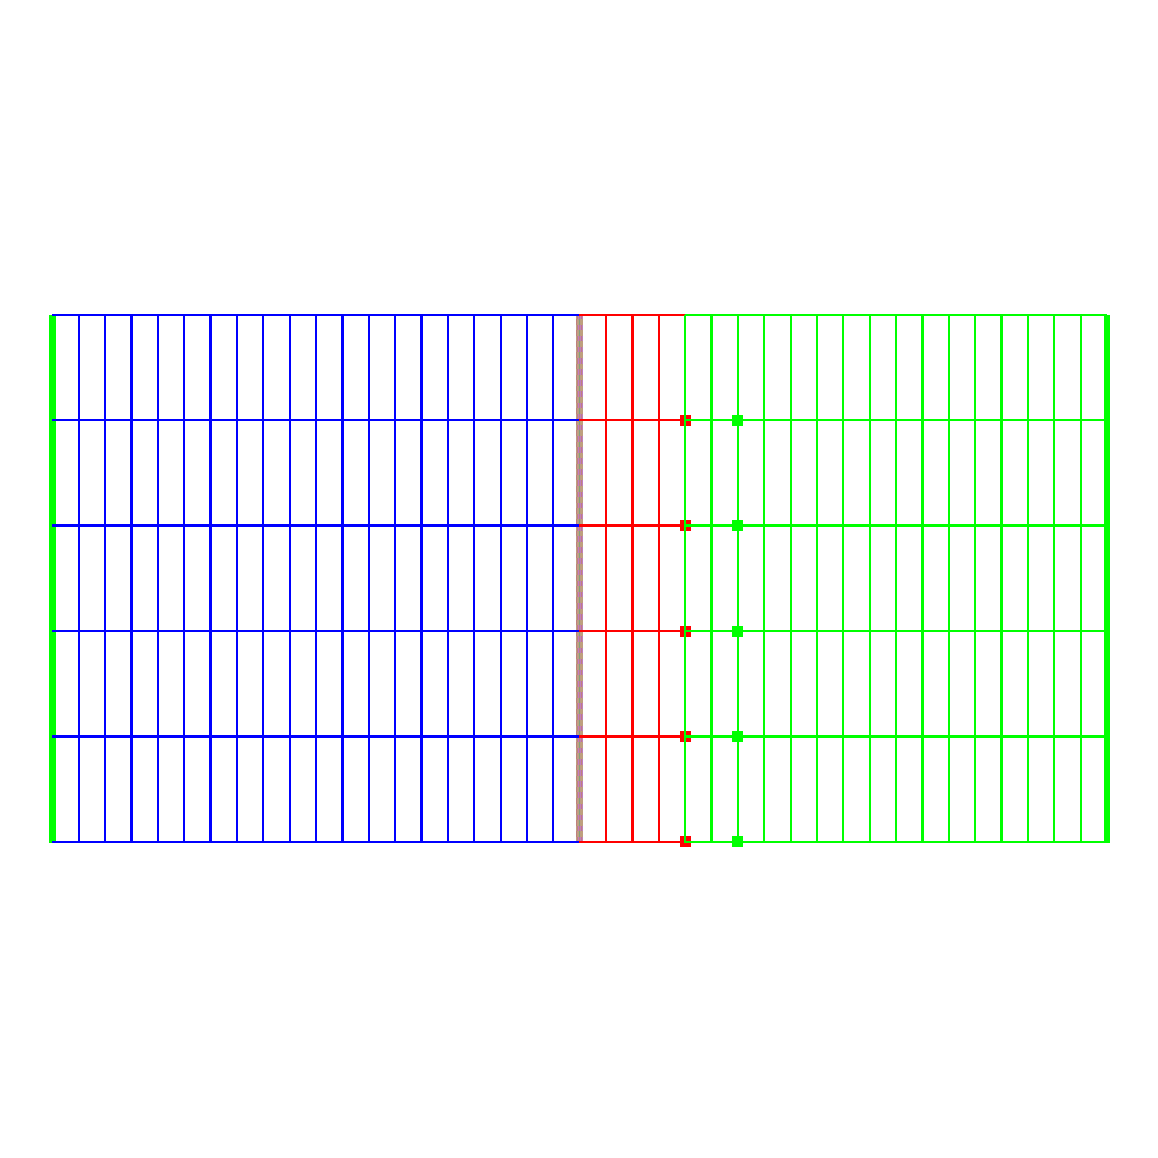
\includegraphics[width=12cm]{planeInterfacenp2Grid.ps}
\caption{Grid for the fluid-solid piston problem. }
\label{fig:fluidSolidPistonGrid}
\end{figure}

Figure~\ref{fig:fluidSolidPiston} shows some results.

\input fluidSolidPistonFig


% -------------------------------------------------------------------------------------------------
\clearpage
\section{Fluid-cavity results}


\input fluidCavityFig.tex




\bibliography{\homeHenshaw/papers/henshaw}
\bibliographystyle{siam}


 \printindex

\end{document}
